% \vspace{-12pt}
\section{Introduction} \label{sec:intro}
As a result of recent advances in machine learning and computer vision, deep neural networks (DNNS) has become an essential part of our lives. DNNs are used to suggest articles to read, detect people in surveillance cameras, automate big machines in factories, and even diagnose X-rays for patients in hospitals. So What is the catch here? These DNNs struggle from a detrimental weakness on specific naive scenarios, despite having a strong performance on average. \figLabel{\ref{fig:intro_fig}} shows how a small perturbation on the view angle of the teapot object results in a drop in InceptionV3 \cite{inception} confidence score from 100\% to almost 0\%. The \emph{softmax} confidence scores are plotted against one semantic parameter (\ie, the azimuth angle around the teapot) and it fails in such a simple task. Similar behaviors are consistently observed across different DNNs (trained on ImageNet \cite{IMAGENET}). \figLabel{\ref{fig:global}} shows that even after averaging over different shapes, we observe a similar behaviour, but with less severity.

\begin{figure}[t]
\tabcolsep=0.03cm
   \begin{tabular}{cccc}
   angle:\ang{122} & angle:\ang{113} & angle:\ang{68} & angle:\ang{55} \\
    \textcolor{green}{teapot:98.22\%} &\textcolor{red}{teapot:0.01\%} &\textcolor{red}{teapot:0.01\%} &\textcolor{green}{teapot:99.89\%} \\ 
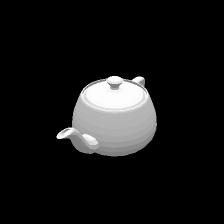
\includegraphics[trim={1.5cm 1.5cm 1.5cm 1.5cm},clip, width = 2cm]{images/intro/class_122.jpg} &
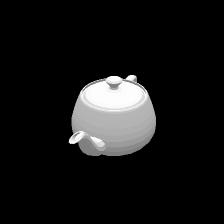
\includegraphics[trim={1.5cm 1.5cm 1.5cm 1.5cm},clip, width = 2cm]{images/intro/class_113.jpg}&
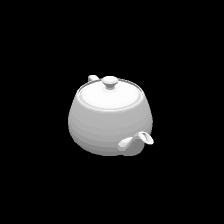
\includegraphics[trim={1.5cm 1.5cm 1.5cm 1.5cm},clip, width = 2cm]{images/intro/class_68.jpg} &
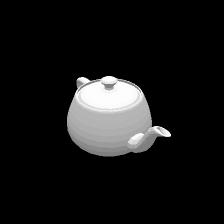
\includegraphics[trim={1.5cm 1.5cm 1.5cm 1.5cm},clip, width = 2cm]{images/intro/class_55.jpg} \\
\end{tabular}
      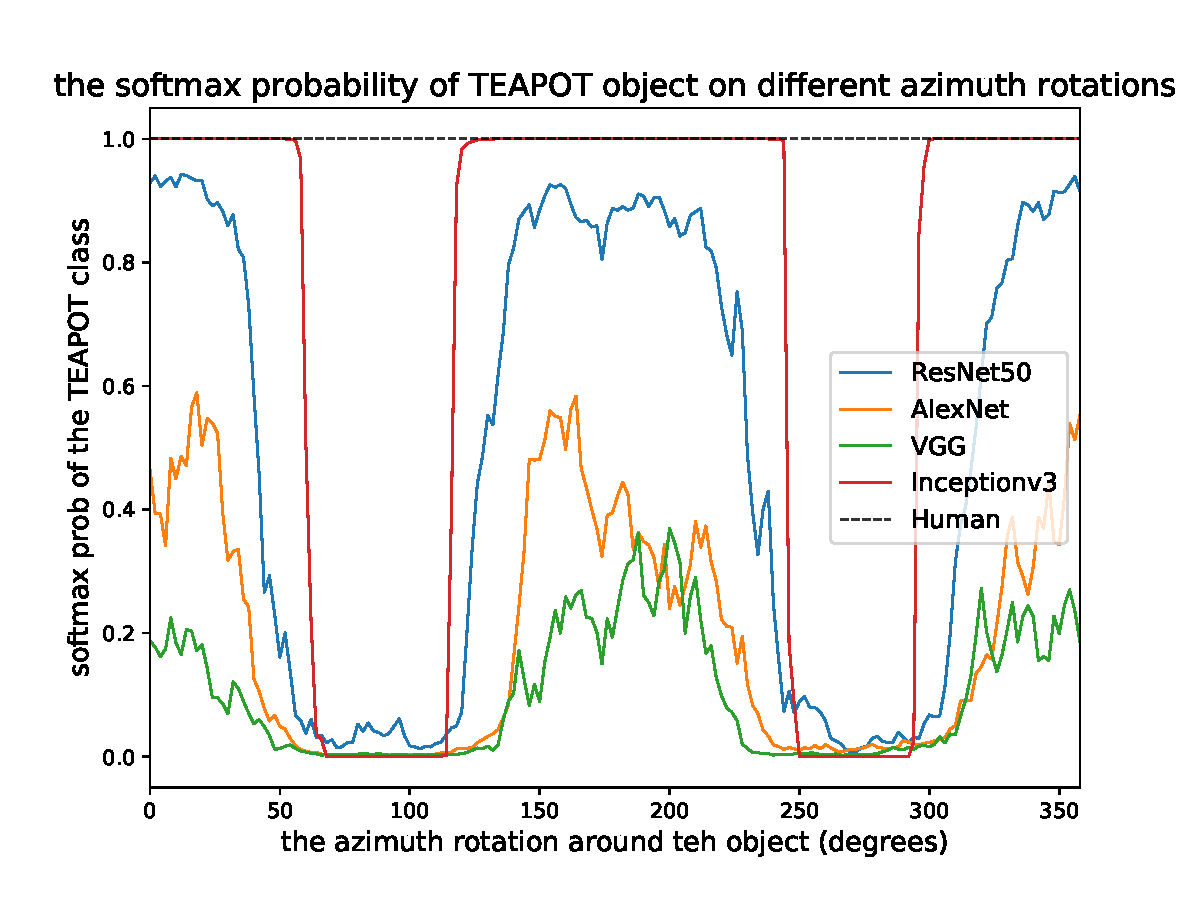
\includegraphics[trim={0.7cm 1.2cm 0.7cm 0.7cm},clip, width=\columnwidth]{images/azimuth_performance_TEAPOT.pdf}\\
       \small \small \tab The azimuth angle around the TEAPOT object (degrees)
       \vspace{-9pt}
   \caption{\small \textbf{Semantic Robustness of Deep Networks}. Trained Neural networks can perform poorly for small perturbations in the semantics of the image. (\textit{top}):We show how for a simple teapot object, perturbing the azimuth view angle of the object can dramatically affect the score of InceptionV3 \cite{inception} score of the teapot class. (\textit{bottom}):We show a plot of the softmax confidence scores of different DNNs on the the same teapot object viewed from 360 degrees around the object. For comparison, Lab researchers identified the object from all angles (18 equally spaced samples)}
   \vspace{-8pt}
   \label{fig:intro_fig}
\end{figure}

Furthermore, because DNNs are not easily interpretable, they work well without a complete understanding of \textit{why} they behave in such manner. A whole direction of research is dedicated to study and analyze DNNs. Examples of such analysis is activation visualization \cite{unn-visual1,unn-visual3,unn-visual2}, noise injection \cite{unn-robustness-noise1,unn-universal,unn-modar}, and studying effect of image manipulation on DNNs \cite{unn-texture,unn-texture,unn-robustness-geometry}. We provide a new lens of semantic robustness analysis of such DNNs as can be seen in \figLabel{\ref{fig:intro_fig}} and subsequent figures. These Network Semantic Maps (NSM) demonstrate unexpected behavior of some DNNs in which adversarial regions lies inside a very confident region of the semantic space, which constitutes a ``trap'' that is hard to detect without such analysis and can lead to catastrophic failure of the DNN.

Recent work in the adversarial attacks explores the DNNs' sensitivity and perform gradient updates to derive targeted perturbations \cite{first-attack,fast-sign,carlini,projected-gradient}. In practice, such attacks are less likely to naturally occur than semantic attacks, such as changes in camera viewpoint and lighting conditions. The literature on semantic attacks is sparser since they are more subtle and challenging to analyze \cite{normal-light-attack,sada}. This is due to the fact we are not able to distinguish between failure cases that result from the network structure, and learning, or from the data bias \cite{bias}. The current methods for adversarial semantic attacks either work on individual examples \cite{strike}, or try to find distributions but rely on sampling methods which do not scale with dimensionality \cite{sada}. We present a novel approach to finds robust/adversarial regions in the n-dimensional semantic space that scale better than sampling-based methods\cite{sada}, and we use such algorithm to quantify semantic robustness of popular DNNs on a collected dataset.

\mysection{Contributions}
\textbf{(1)} We analyze the networks on the semantic lens showing unexpected behavior in the 1,2D semantic space. \textbf{(2)} We develop a new method to detect regions in the semantic space that the DNN behaves robustly/poorly that scale well with increasing dimensions (unlike other sampling-based methods). The method is optimization based and follows rigorously from optimizing the bounds around a point of interest. \textbf{(3)} We develop a new metric to measure semantic robustness of DNNs that we dub Semantic Robustness Volume Ratio (SRVR), and we use it to benchmark famous DNNs on a collected dataset. 
\begin{figure}[t]
    \centering
  \includegraphics[width=\columnwidth]{images/average_azimuth_performance_TOILET.pdf}
  \vspace{-8pt}
  \caption{\small \textbf{Class Global Adversarial Regions}: average scores on $10$ different shapes from the toilet class. We can see these semantic regions are shared among different shapes of that specific class as well as by different DNNs.}
  \label{fig:global}
  \vspace{-4pt}
\end{figure}
